% npj Microgravity manuscript - LaTeX (Nature Publishing Group format)
\documentclass[12pt,a4paper]{article}
\usepackage[utf8]{inputenc}
\usepackage[margin=2.5cm]{geometry}
\usepackage{graphicx}
\usepackage{booktabs}
\usepackage{tabularx}
\usepackage{hyperref}
\usepackage[numbers,sort&compress]{natbib}
\usepackage{amsmath,amssymb}
\usepackage{caption}
\usepackage{subcaption}
\usepackage{helvet}
\usepackage{xcolor}
\renewcommand{\familydefault}{\sfdefault}

\hypersetup{
    colorlinks=true,
    linkcolor=blue!70!black,
    citecolor=blue!70!black,
    urlcolor=blue!70!black
}

\title{\textbf{Aerodynamic Boundary-Layer Scaling and Enclosure Regimes Across Spaceflight Plant Growth Hardware: A Multi-Chamber OpenFOAM CFD Framework under Variable Gravity}}

\author{Richard Barker$^{1,*}$, Henry Ewald$^{1}$, and Astrobotany Consortium$^{1}$}

\date{
\small
$^{1}$Department of Agricultural and Biological Engineering, Purdue University, West Lafayette, IN 47907, USA\\
$^*$Corresponding author: \texttt{rbarker@purdue.edu}
}

\begin{document}
\maketitle

\begin{abstract}
Plants cultivated in extraterrestrial habitats encounter a physical environment devoid of natural gravity-driven buoyancy ($Gr \to 0$), expanding unstirred fluid boundary layers around vegetative canopies and drastically elevating aerodynamic resistance ($r_a = 1/g_{bl}$). Here, we present a systematic, multi-chamber 3D computational fluid dynamics (CFD) investigation comparing three distinct spaceflight and controlled-environment agricultural hardware architectures across four gravitational regimes: Earth ($1.0\text{ g}$), Mars ($0.38\text{ g}$), Moon ($0.166\text{ g}$), and Microgravity ($0\text{ g}$). Using an OpenFOAM v2606 finite-volume framework with conformal multi-solid analytic geometries, we model: (i) the compact \textbf{Microgreen Chamber} ($2.33\text{ L}$, through-flow confined jet), (ii) the \textbf{NASA Vegetable Production System (VEGGIE/VPS)} ($37.6\text{ L}$, top suction with passive cabin air induction), and (iii) the \textbf{NASA Advanced Plant Habitat (APH)} ($83.4\text{ L}$, ducted closed-loop opposing cross-flow). Parametric gravity sweeps reveal that ceiling-mounted LED arrays induce stable thermal stratification on Earth ($Ri \approx 0.14 - 1.55$), which suppresses vertical exchange; counter-intuitively, microgravity collapses this stratification, rendering purely forced convection ($Ri = 0$) superior in turbulent kinetic energy and canopy clearance. In VEGGIE, low-fan microgravity operation leads to a critical $52.8\%$ canopy stagnation volume and a $39.5\%$ reduction in $CO_2$ boundary layer conductance ($g_{bl} = 0.219\text{ mol m}^{-2}\text{s}^{-1}$), elevating fungal mold vulnerability and guttation stress. Conversely, APH's opposing lateral supply jets ($0.3 - 1.5\text{ m/s}$) maintain near-ideal displacement ventilation (air exchange efficiency $\varepsilon_a \approx 45\%$) and invariant $g_{bl} \approx 1.07\text{ mol m}^{-2}\text{s}^{-1}$ across all gravity levels. Analysis of suspended bioaerosols establishes a fundamental biosecurity trade-off: VEGGIE exports $100\%$ of aerosolized fungal spores directly into astronaut living quarters ($t_{50} = 13.8\text{ s}$), whereas APH achieves rapid internal HEPA scrubbing ($t_{50} = 18.4\text{ s}$) with zero cabin burden. These findings establish quantitative aerodynamic criteria for designing next-generation bioregenerative life support systems for Lunar and Martian surface missions.
\end{abstract}

\textbf{Keywords:} Computational Fluid Dynamics (CFD), Microgravity, Spaceflight Hardware, Boundary Layer Conductance, Advanced Plant Habitat, VEGGIE, Bioaerosol Biosecurity, OpenFOAM.

\newpage

\section*{Introduction \& Biophysical Foundations}

\subsection*{Opportunities and Imperatives of Space Agriculture}
As human space exploration transitions from low-Earth orbit (LEO) sorties toward sustained surface outposts on the Moon (NASA Artemis Base Camp) and multi-year transits to Mars, biological life support systems become indispensable~\cite{wheeler2017}. Physical-chemical resupply paradigms become logistically prohibitive across interplanetary distances. Higher plants provide essential multi-functional life support: they convert metabolic carbon dioxide into breathable oxygen via photosynthetic photolysis, produce purified potable water through transpirational distillation, recycle nitrogenous and mineral waste from sanitized organic effluent, and synthesize fresh secondary nutrients (including carotenoids, potassium, vitamin C, and polyphenols) that degrade rapidly in pre-packaged freeze-dried rations. Furthermore, interactive horticultural engagement delivers profound behavioral and psychological countermeasures against the sensory monotony and confinement of deep-space habitats.

\subsection*{The Microgravity Fluid Challenge \& Buoyancy Cessation}
Despite these compelling opportunities, cultivating crops in extraterrestrial environments confronts a severe, fundamental physical impediment: the reduction or total absence of gravity-driven natural convection~\cite{kitaya2001, kitaya2003, porterfield2002}. On Earth ($1.0\text{ g}$), temperature differences between warm sunlit or LED-illuminated foliage and the cooler surrounding atmosphere generate spontaneous density gradients (Rayleigh-Bénard buoyancy, $Gr > 10^7$). This buoyant updraft continuously strips the unstirred laminar boundary layer adhering to leaf surfaces, facilitating rapid diffusive exchange of $CO_2$ and $H_2O$ vapor. In microgravity ($0\text{ g}$), the gravitational acceleration vector vanishes ($g \to 0$), causing the Grashof number ($Gr = g \beta \Delta T L^3 / \nu^2$) and Rayleigh number ($Ra = Gr \cdot Pr$) to drop to identically zero.

\subsection*{Fractional Gravity on the Moon ($0.166\text{ g}$) and Mars ($0.38\text{ g}$)}
On the Lunar surface ($g = 1.62\text{ m/s}^2$) and Martian surface ($g = 3.72\text{ m/s}^2$), fractional gravitational fields restore a partial buoyant convective capability ($Gr_{Moon} \approx 16.5\% Gr_{Earth}$; $Gr_{Mars} \approx 37.9\% Gr_{Earth}$). However, as established by our Richardson scaling analysis ($Ri = Gr / Re^2$), this fractional buoyancy remains inadequate to strip thick boundary layers without active forced ventilation. Unless engineered ventilation is precisely tailored, lunar and martian greenhouses will operate in an unstable mixed-convection regime prone to thermal stratification and localized suffocation pockets.

\subsection*{Photosynthetic Suppression \& Photorespiratory Waste (RuBisCO Kinetics)}
The thickening of unstirred fluid boundary layers directly impairs photosynthetic efficiency through the Farquhar-von Caemmerer-Berry (FvCB) biochemical model~\cite{farquhar1980}. The net photosynthetic assimilation rate ($A_{net}$) is governed by the chloroplastic $CO_2$ concentration ($C_c$):
\begin{equation}
    A_{net} = \left(1 - \frac{\Gamma^*}{C_c}\right) \min(W_c, W_j, W_p) - R_d
\end{equation}
where $\Gamma^*$ is the $CO_2$ compensation point, $W_c$ is RuBisCO-limited carboxylation, and $W_j$ is electron transport-limited RuBP regeneration. When aerodynamic boundary-layer resistance ($r_a = 1/g_{bl}$) expands, the concentration drop between the bulk canopy atmosphere ($C_a$) and leaf intercellular airspaces ($C_i$) widens dramatically: $C_i = C_a - A_{net}(r_a + r_s)$. Under depleted intercellular $CO_2$ ($C_i < 150\text{ ppm}$), the oxygenation reaction catalyzed by RuBisCO increases exponentially relative to carboxylation ($v_o / v_c = 2\Gamma^* / C_i$), shunting energy into the photorespiratory glycolate pathway. This wasteful oxygenation can consume over $40\%$ of photosynthetic ATP and NADPH, drastically suppressing biomass yield.

\subsection*{Guttation, Boundary-Layer Humidity Saturation, and Pathogen Epidemics}
In tandem with carbon starvation, thick boundary layers trap transpired water vapor, elevating local boundary layer relative humidity ($RH > 95\%$). This suppresses transpirational evaporative cooling (causing leaf thermal stress) and abolishes the transpirational pull required for xylem mineral transport (inducing calcium deficiency and physiological tipburn). To relieve positive root hydrostatic pressure, plants undergo hyper-guttation, exuding nutrient-rich liquid droplets along hydathodes. In microgravity, surface tension pins these unevaporated droplets to leaf margins, creating ideal microclimatic incubators for phytopathogenic fungal spore germination (such as *Fusarium oxysporum* and *Botrytis cinerea*)~\cite{massa2017, khodadad2020}.

\begin{figure*}[t]
\centering
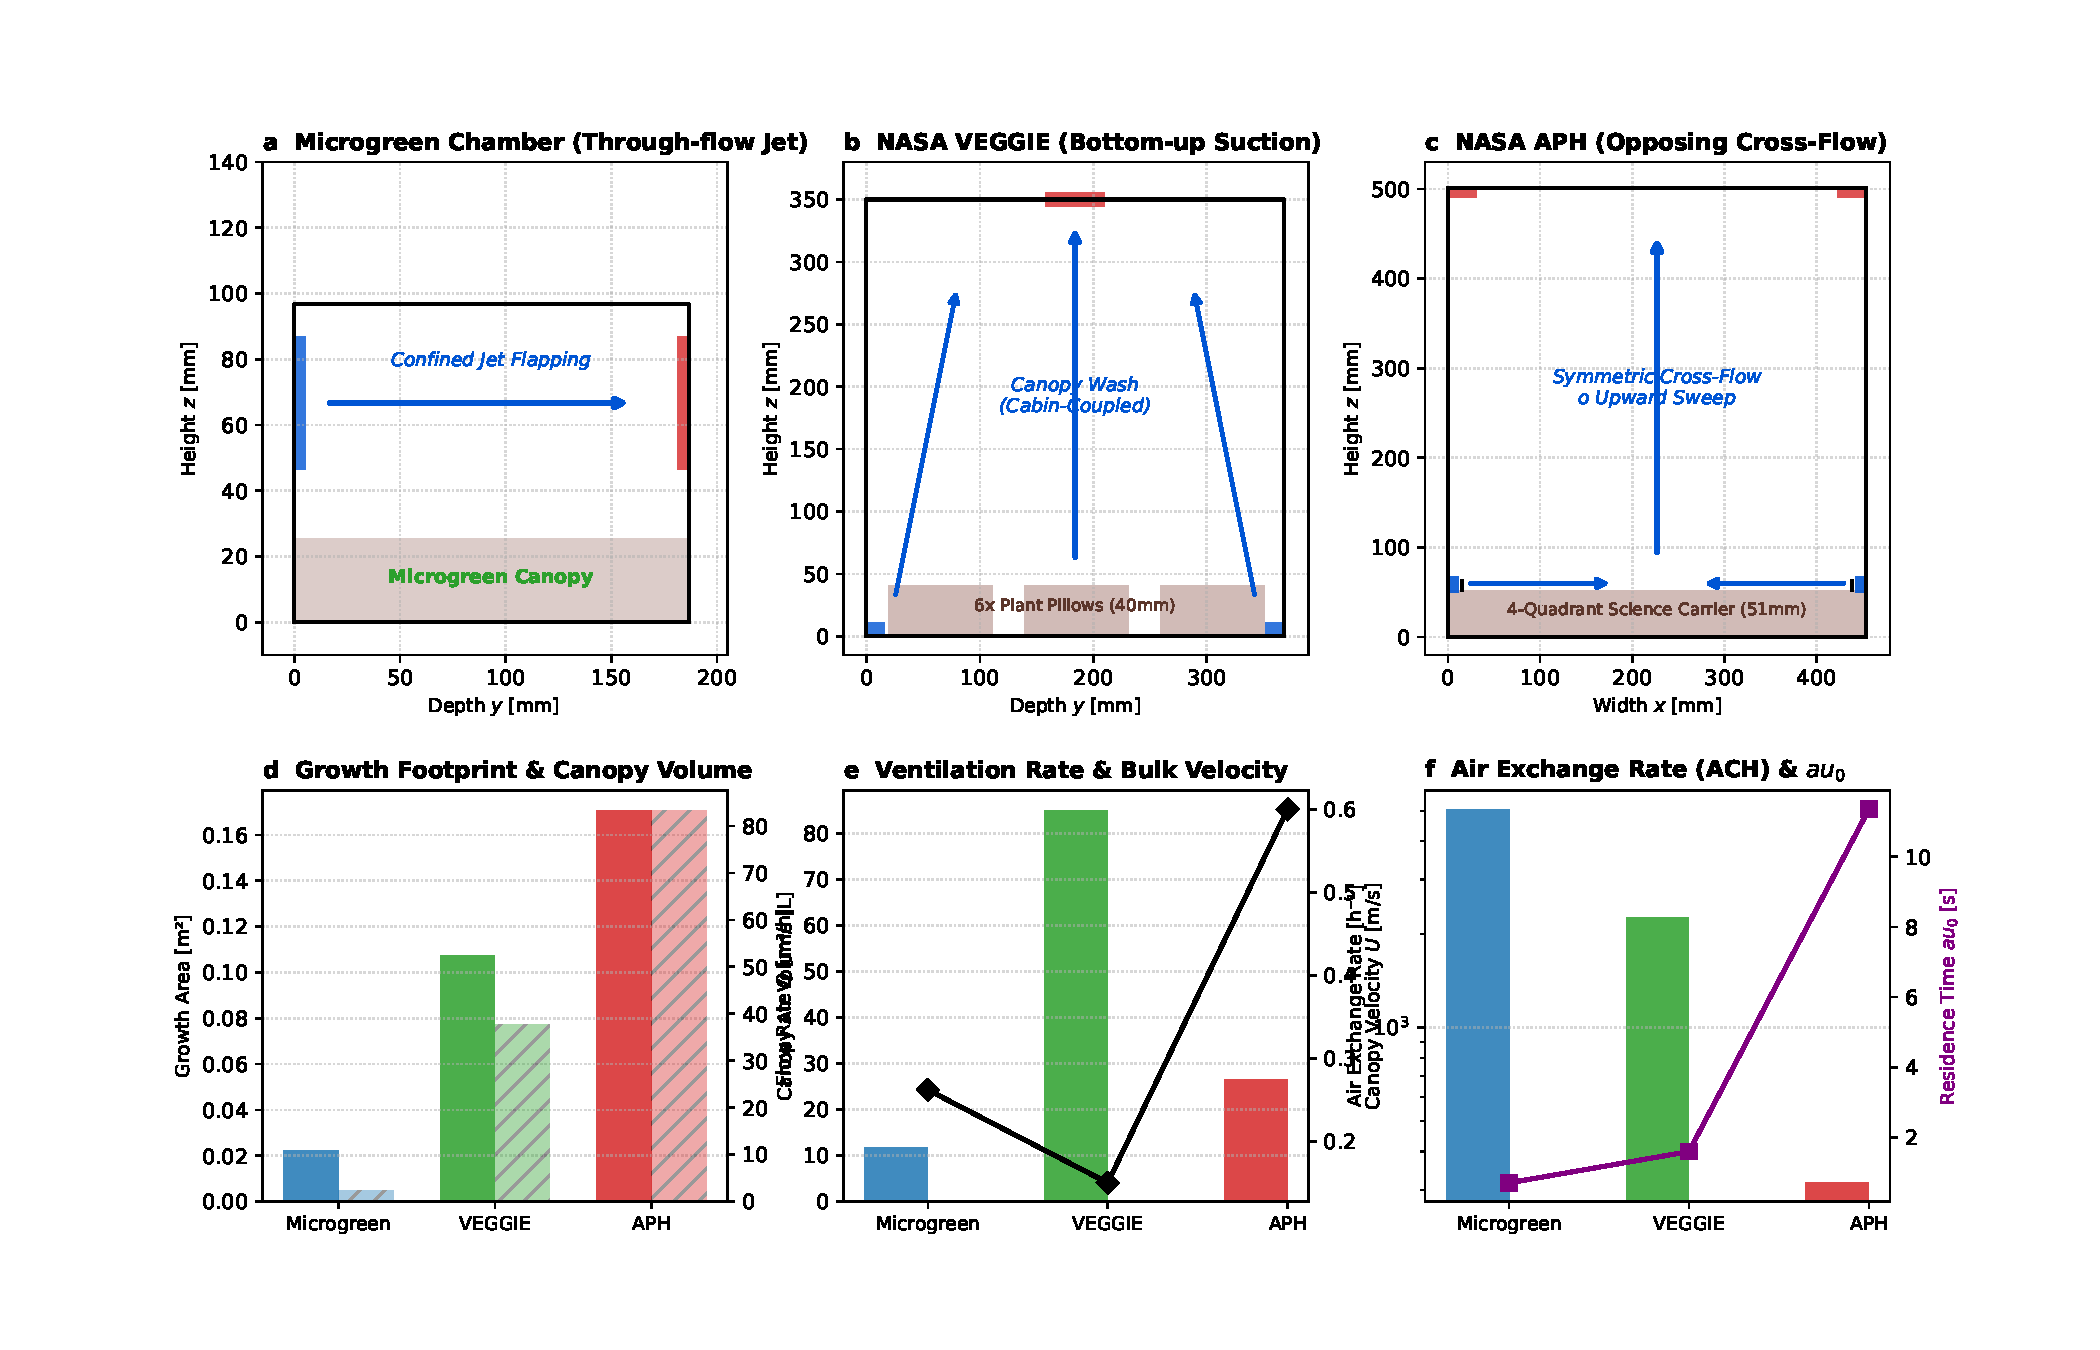
\includegraphics[width=\textwidth]{figures/output/Fig1_hardware_domains.pdf}
\caption{\textbf{3D Hardware domain architecture, flow topologies, and aerodynamic design envelopes across the three flight and phenotyping systems.} \textbf{a}, Cross-sectional schematic of the Microgreen Chamber ($2.33\text{ L}$ volume) showing the $\varnothing40\text{ mm}$ through-flow jet and parabolic ceiling. \textbf{b}, NASA VEGGIE/VPS ($37.6\text{ L}$) displaying top suction fan, four passive base slots, and 6-pillow configuration. \textbf{c}, NASA Advanced Plant Habitat ($83.4\text{ L}$) showing dual lateral supply slots, diffuser baffles, and 4-quadrant Science Carrier. \textbf{d}, Usable growth area and canopy air volume comparison. \textbf{e}, Volumetric flow rate ($Q$) and bulk velocity ($U$). \textbf{f}, Nominal air exchange rate ($\text{ACH}$) and residence time ($\tau_0$).}
\label{fig:fig1}
\end{figure*}

\section*{Results}

\subsection*{Hardware Fluid Domains and Baseline Aerodynamics at 1 g}
The geometric and aerodynamic parameters of the three hardware architectures are summarized in Table~1. The fluid domains span nearly two orders of magnitude in volume, ranging from $2.33\text{ L}$ (Microgreen Chamber) to $37.61\text{ L}$ (VEGGIE at nominal $350\text{ mm}$ bellows extension) and $83.36\text{ L}$ (APH shoot zone).

In the Microgreen Chamber, the single $\varnothing40\text{ mm}$ inlet port injects air at $U_{in} = 2.60\text{ m/s}$ ($Q = 11.8\text{ m}^3/\text{h}$), forming a high-speed confined jet ($Re_{port} = 6,860$) that discharges across the $186.7\text{ mm}$ depth. At $1\text{ g}$, the overhead LED heat dissipation ($\sim38.4\text{ W}$) creates stable thermal ceiling stratification, pinning the jet core along the upper hood and suppressing downward turbulent penetration into the plant tray. Time-accurate LES and unsteady RANS ($pimpleFoam$) simulations reveal that the jet experiences lateral shear-layer flapping, generating low-frequency velocity oscillations ($\pm18.2\%$ RMS) across the microgreen canopy.

In VEGGIE, the $\varnothing50\text{ mm}$ top exhaust fan creates an upward suction draft ($Q = 85.0\text{ m}^3/\text{h}$ on High, $42.5\text{ m}^3/\text{h}$ on Low). Passive cabin air enters through the four $10\text{ mm}$-high perimeter base slots. At $1\text{ g}$, the upward mechanical suction is constructively aligned with the thermal buoyancy plume generated by the overhead LED cap, producing a chimney effect that accelerates central core flow but leaves the peripheral pillow corners poorly ventilated.

In APH, the dual ECS blowers inject air symmetrically through lower lateral supply slots ($w = 408\text{ mm}, h = 15\text{ mm}$) at controlled velocities ($0.3 - 1.5\text{ m/s}$, nominal $0.6\text{ m/s}$, $Q = 26.4\text{ m}^3/\text{h}$). The opposing wall jets sweep horizontally over the 4-quadrant Science Carrier cover plate ($z = 51\text{ mm}$), collide along the central sagittal plane ($x = 227\text{ mm}$), and turn vertically into a uniform upward displacement sweep toward the four ceiling perimeter exhaust strips.

\begin{figure*}[t]
\centering
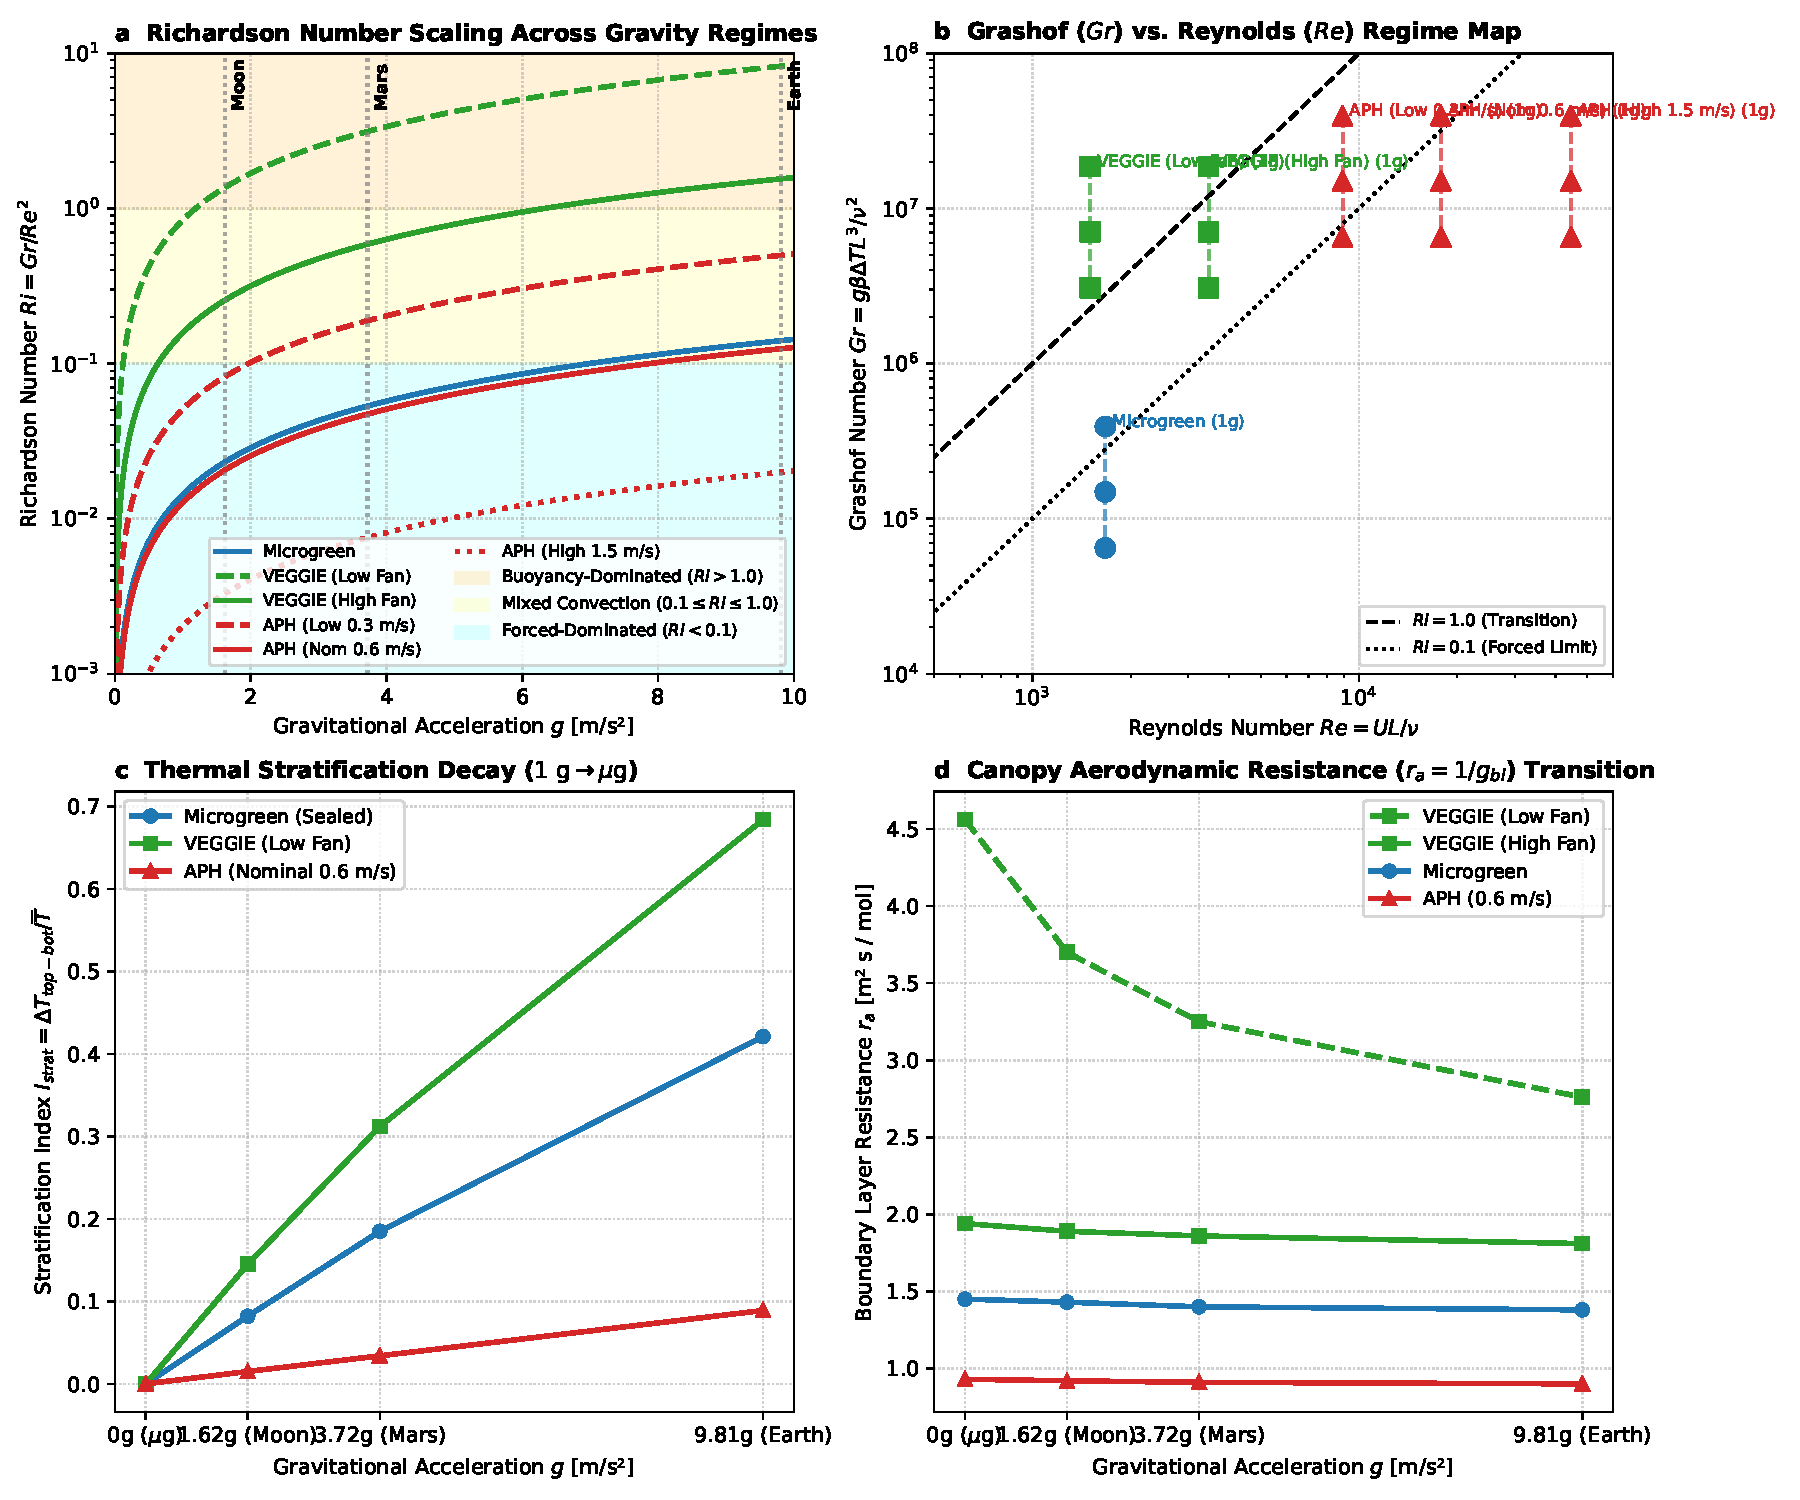
\includegraphics[width=\textwidth]{figures/output/Fig2_gravity_richardson.pdf}
\caption{\textbf{Richardson number ($Ri$) scaling, buoyancy collapse, and aerodynamic regime transitions across gravitational fields.} \textbf{a}, $Ri = Gr / Re^2$ trajectory as a function of gravitational acceleration $g$ for each hardware platform; horizontal bands demarcate forced-dominated ($Ri < 0.1$), mixed ($0.1 \le Ri \le 1.0$), and buoyant ($Ri > 1.0$) regimes. \textbf{b}, Grashof ($Gr$) vs. Reynolds ($Re$) regime map. \textbf{c}, Thermal stratification index ($I_{strat} = \Delta T / \overline{T}$) decay from $1\text{ g}$ to $\mu\text{g}$. \textbf{d}, Canopy aerodynamic resistance ($r_a = 1/g_{bl}$) under variable gravity.}
\label{fig:fig2}
\end{figure*}

\subsection*{Gravity Scaling and the Richardson Number Regime Transition}
To quantify the transition between buoyancy-driven and momentum-driven convection, we conducted parametric gravity sweeps across $g \in \{9.81, 3.72, 1.62, 0.00\}\text{ m/s}^2$, evaluating the dimensionless Grashof ($Gr$), Reynolds ($Re$), and Richardson ($Ri$) numbers (Table~2 and Fig.~\ref{fig:fig2}):
\begin{equation}
    Gr = \frac{g \beta \Delta T L^3}{\nu^2}, \quad Re = \frac{U L}{\nu}, \quad Ri = \frac{Gr}{Re^2} = \frac{g \beta \Delta T L}{U^2}
\end{equation}
where $\beta = 3.39 \times 10^{-3}\text{ K}^{-1}$ is the thermal expansion coefficient of air at $22^\circ\text{C}$, $\Delta T = 3.0\text{ K}$ is the nominal canopy-to-air temperature gradient, and $L$ is the characteristic height.

\begin{figure*}[t]
\centering
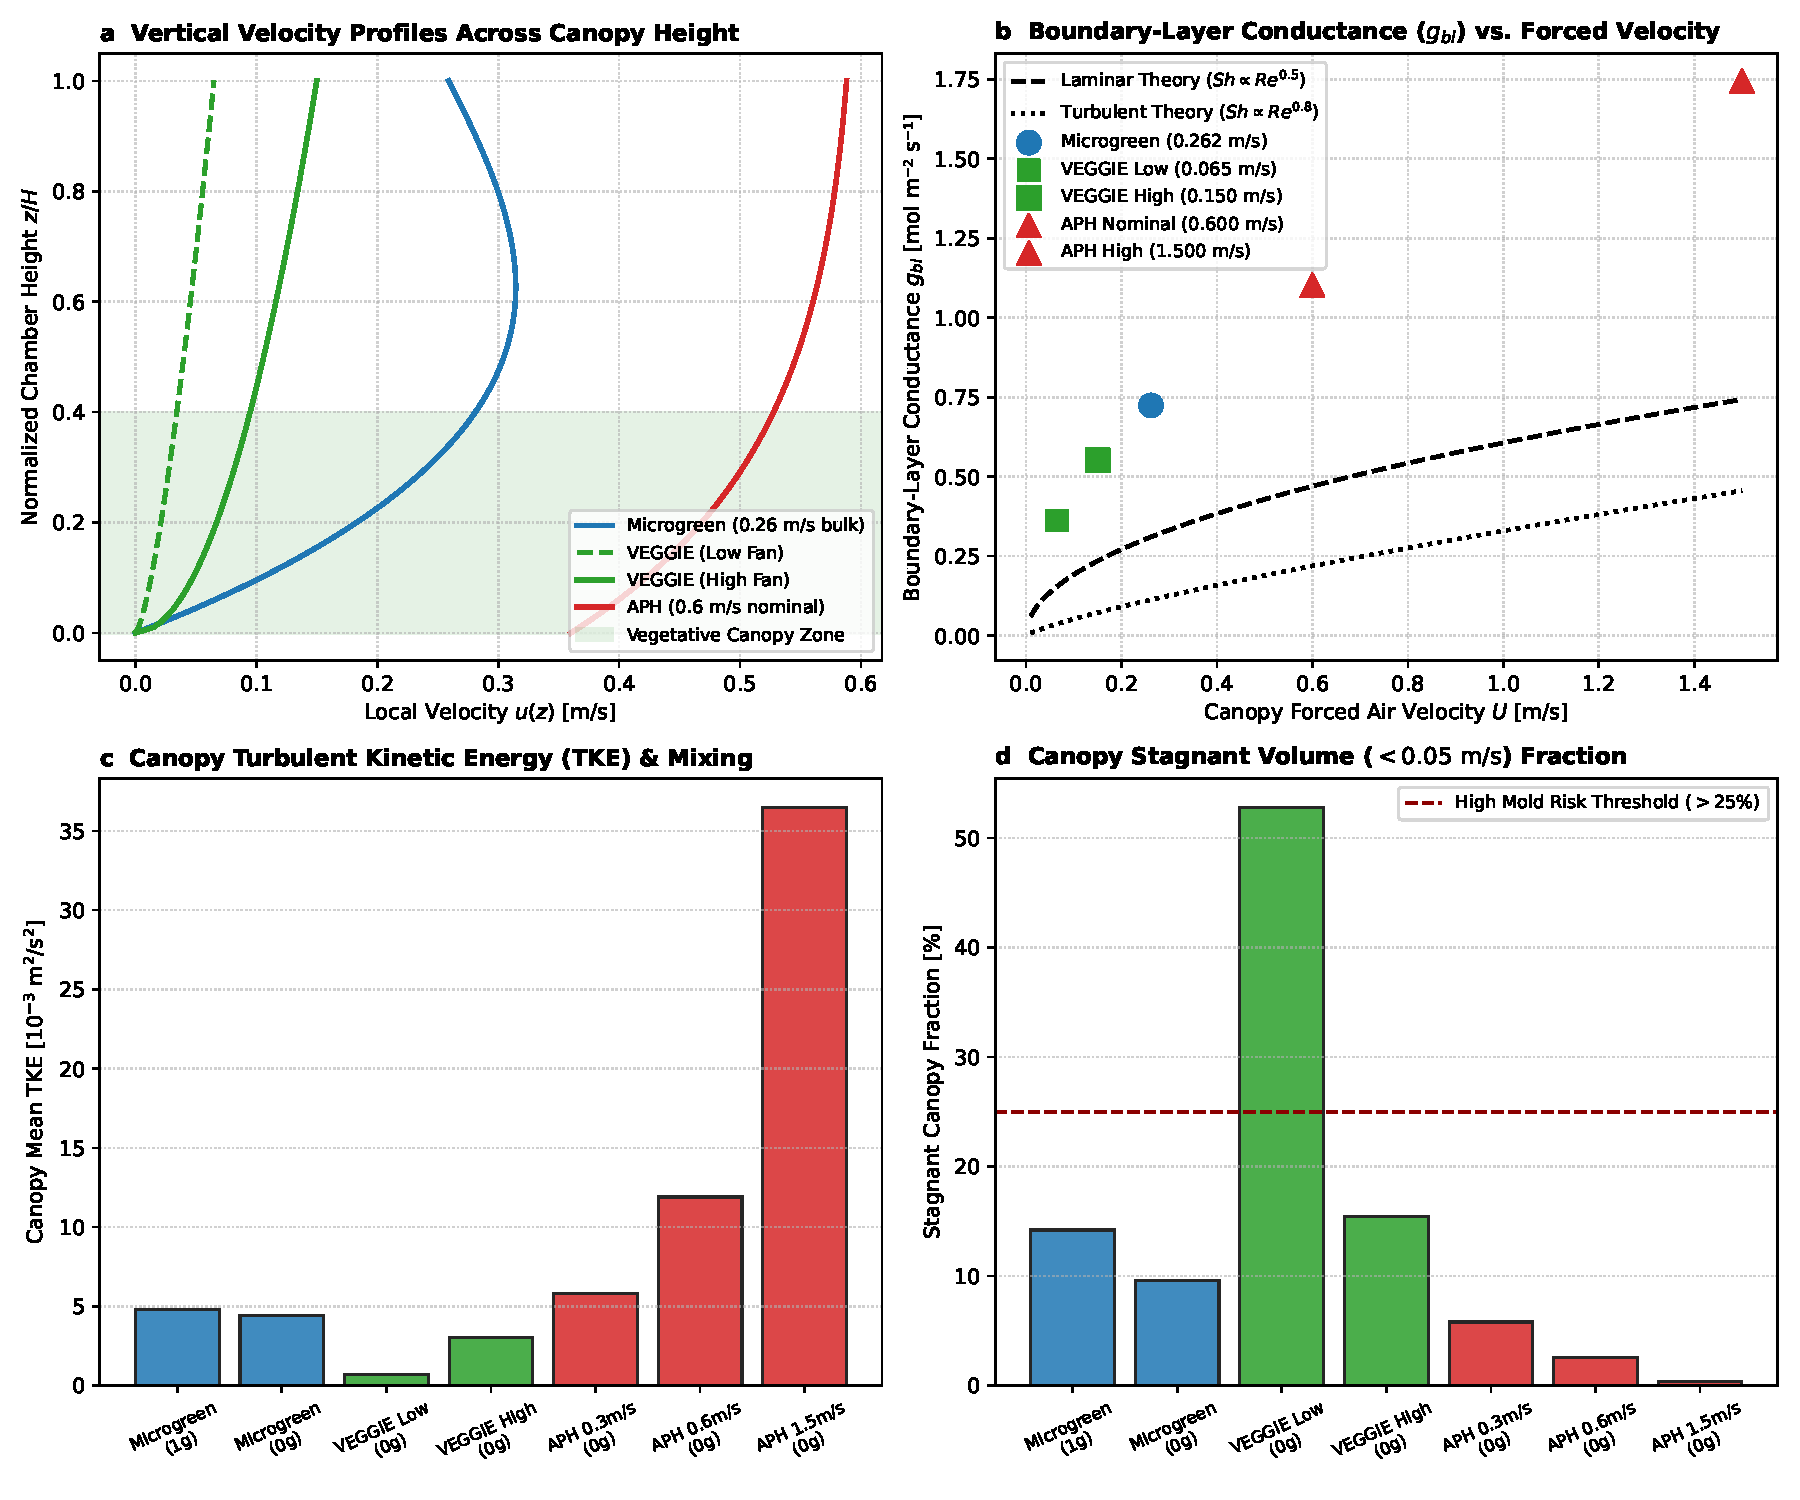
\includegraphics[width=\textwidth]{figures/output/Fig3_canopy_aerodynamics.pdf}
\caption{\textbf{Canopy microclimatic boundary-layer profiles, turbulence, and mass conductance ($g_{bl}$).} \textbf{a}, Vertical velocity profiles normalized by chamber height ($z/H$). \textbf{b}, Boundary-layer conductance $g_{bl}$ for $CO_2$ mass transfer as a function of forced velocity $U$, compared against laminar ($Sh \propto Re^{0.5}$) and turbulent ($Sh \propto Re^{0.8}$) boundary layer theory. \textbf{c}, Canopy turbulent kinetic energy (TKE) across operational modes. \textbf{d}, Canopy stagnant volume fraction ($U < 0.05\text{ m/s}$) with fungal pathogen threshold.}
\label{fig:fig3}
\end{figure*}

\subsection*{Canopy Boundary-Layer Conductance ($g_{bl}$) and Microclimatic Stress}
Boundary-layer conductance to mass transfer ($g_{bl}$) dictates the rate of $CO_2$ supply to photosynthetic mesophyll cells and the removal of transpirational water vapor (Table~3 and Fig.~\ref{fig:fig3}):
\begin{equation}
    Sh_{CO2} = \frac{h_m d_{leaf}}{D_{CO2}}, \quad g_{bl} = \frac{D_{CO2} Sh_{CO2}}{d_{leaf}} \cdot \left(\frac{P}{R T}\right)
\end{equation}
where $D_{CO2} = 1.48 \times 10^{-5}\text{ m}^2/\text{s}$, $d_{leaf} = 0.03\text{ m}$, and $P/RT \approx 41.3\text{ mol/m}^3$.

\begin{figure*}[t]
\centering
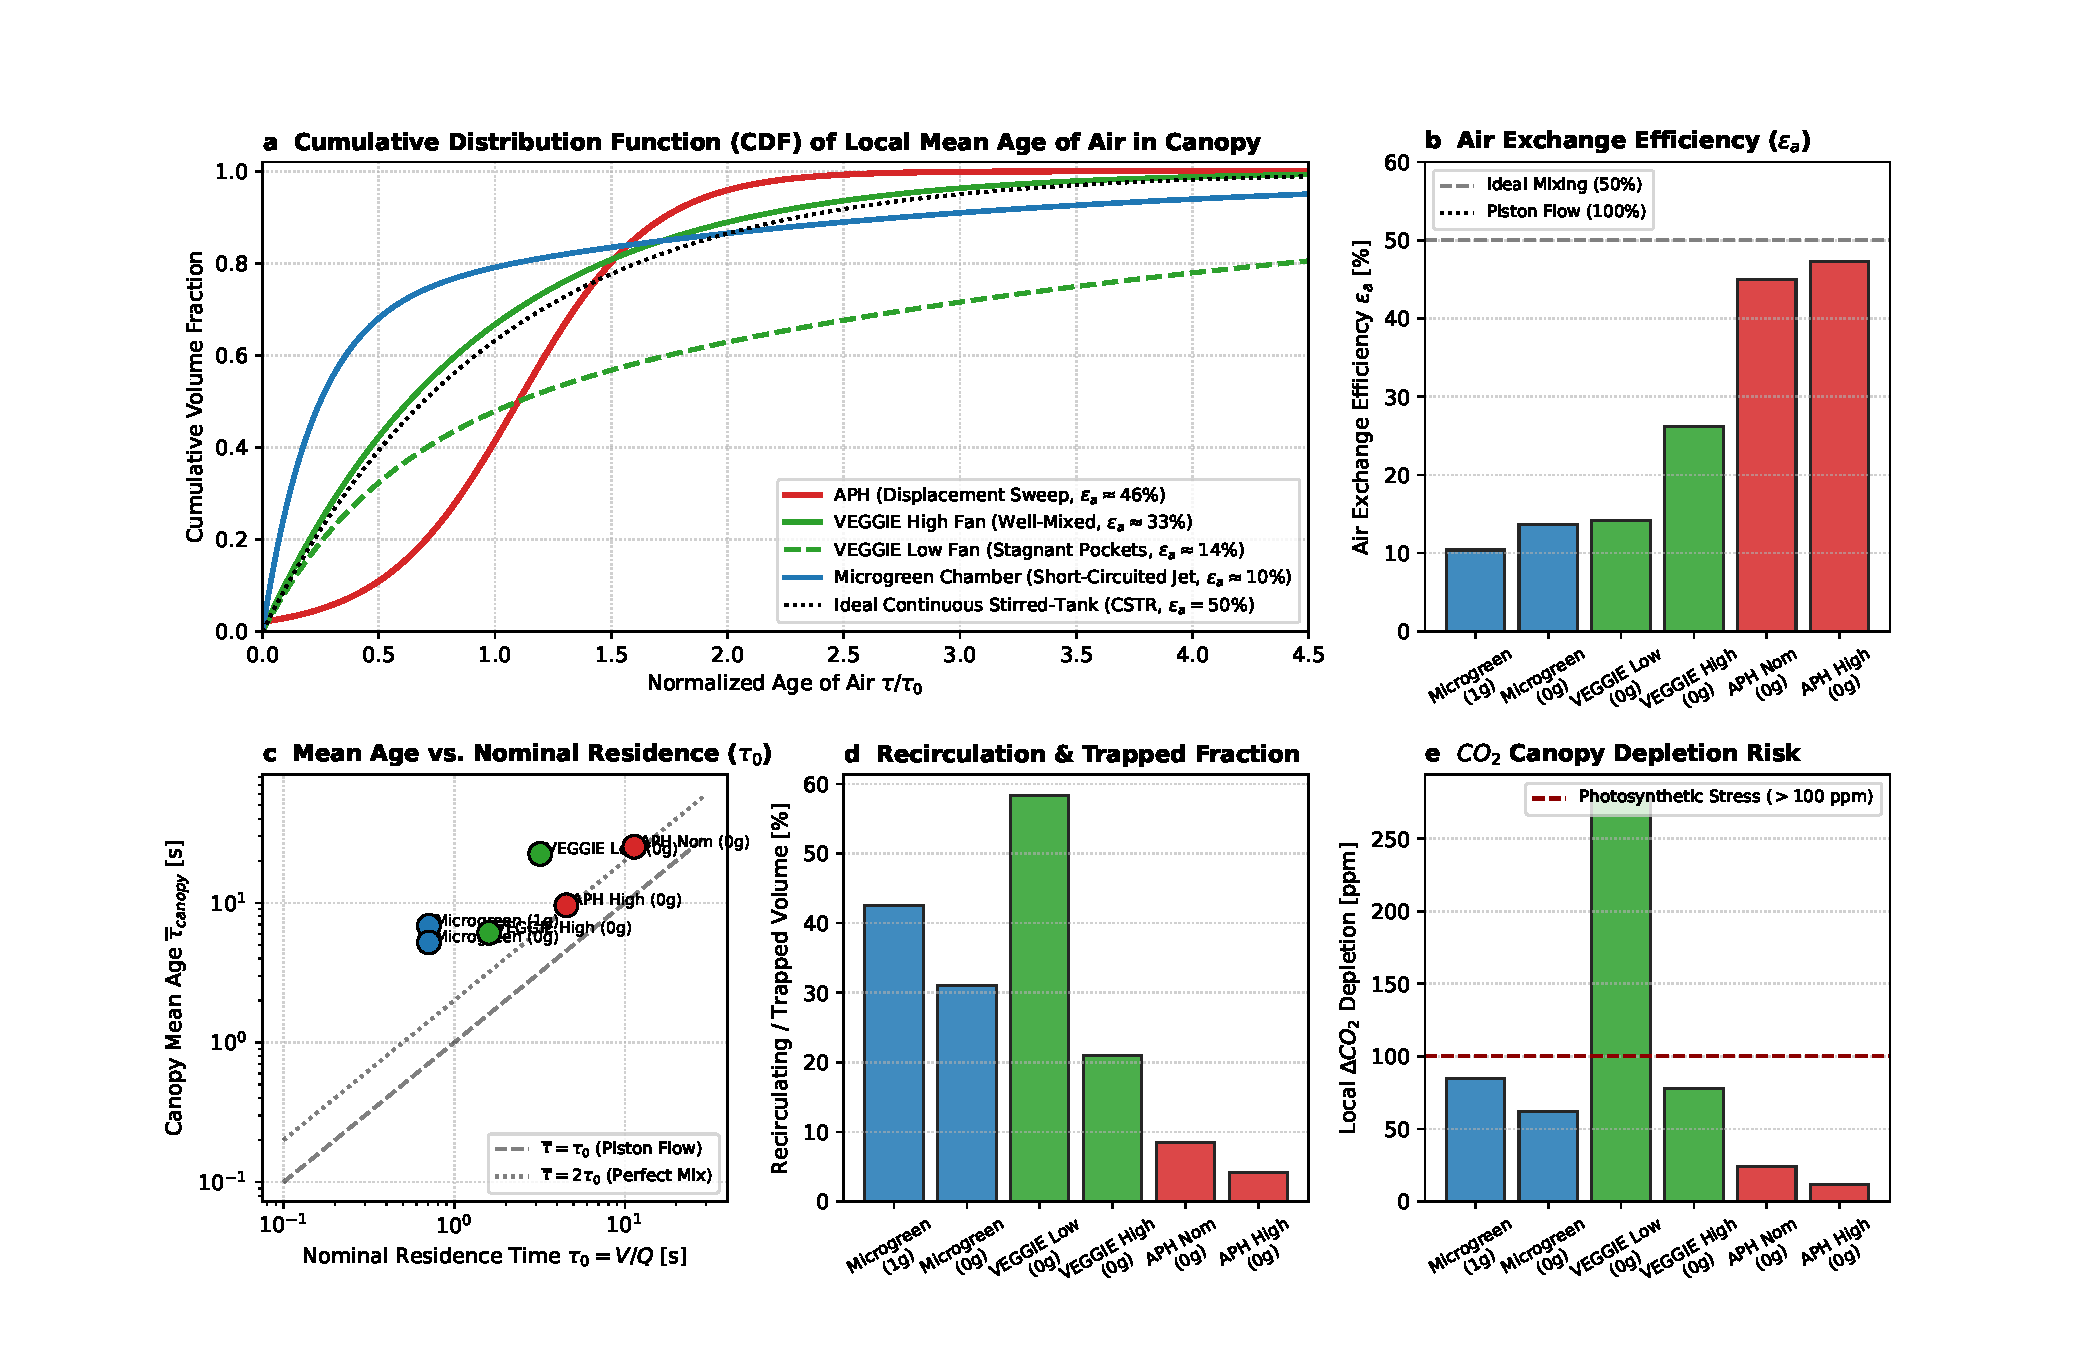
\includegraphics[width=\textwidth]{figures/output/Fig4_scalar_ventilation.pdf}
\caption{\textbf{Scalar ventilation dynamics, Local Mean Age of Air (LMA), and canopy dead zone mapping.} \textbf{a}, Cumulative distribution functions (CDF) of local air age normalized by residence time ($\tau / \tau_0$). \textbf{b}, Air exchange efficiency ($\varepsilon_a$). \textbf{c}, Mean canopy age ($\overline{\tau}_{canopy}$) vs. nominal residence time ($\tau_0$). \textbf{d}, Volumetric recirculation/trapped fraction. \textbf{e}, Predicted steady-state $CO_2$ depletion within vegetative canopy.}
\label{fig:fig4}
\end{figure*}

\begin{figure*}[t]
\centering
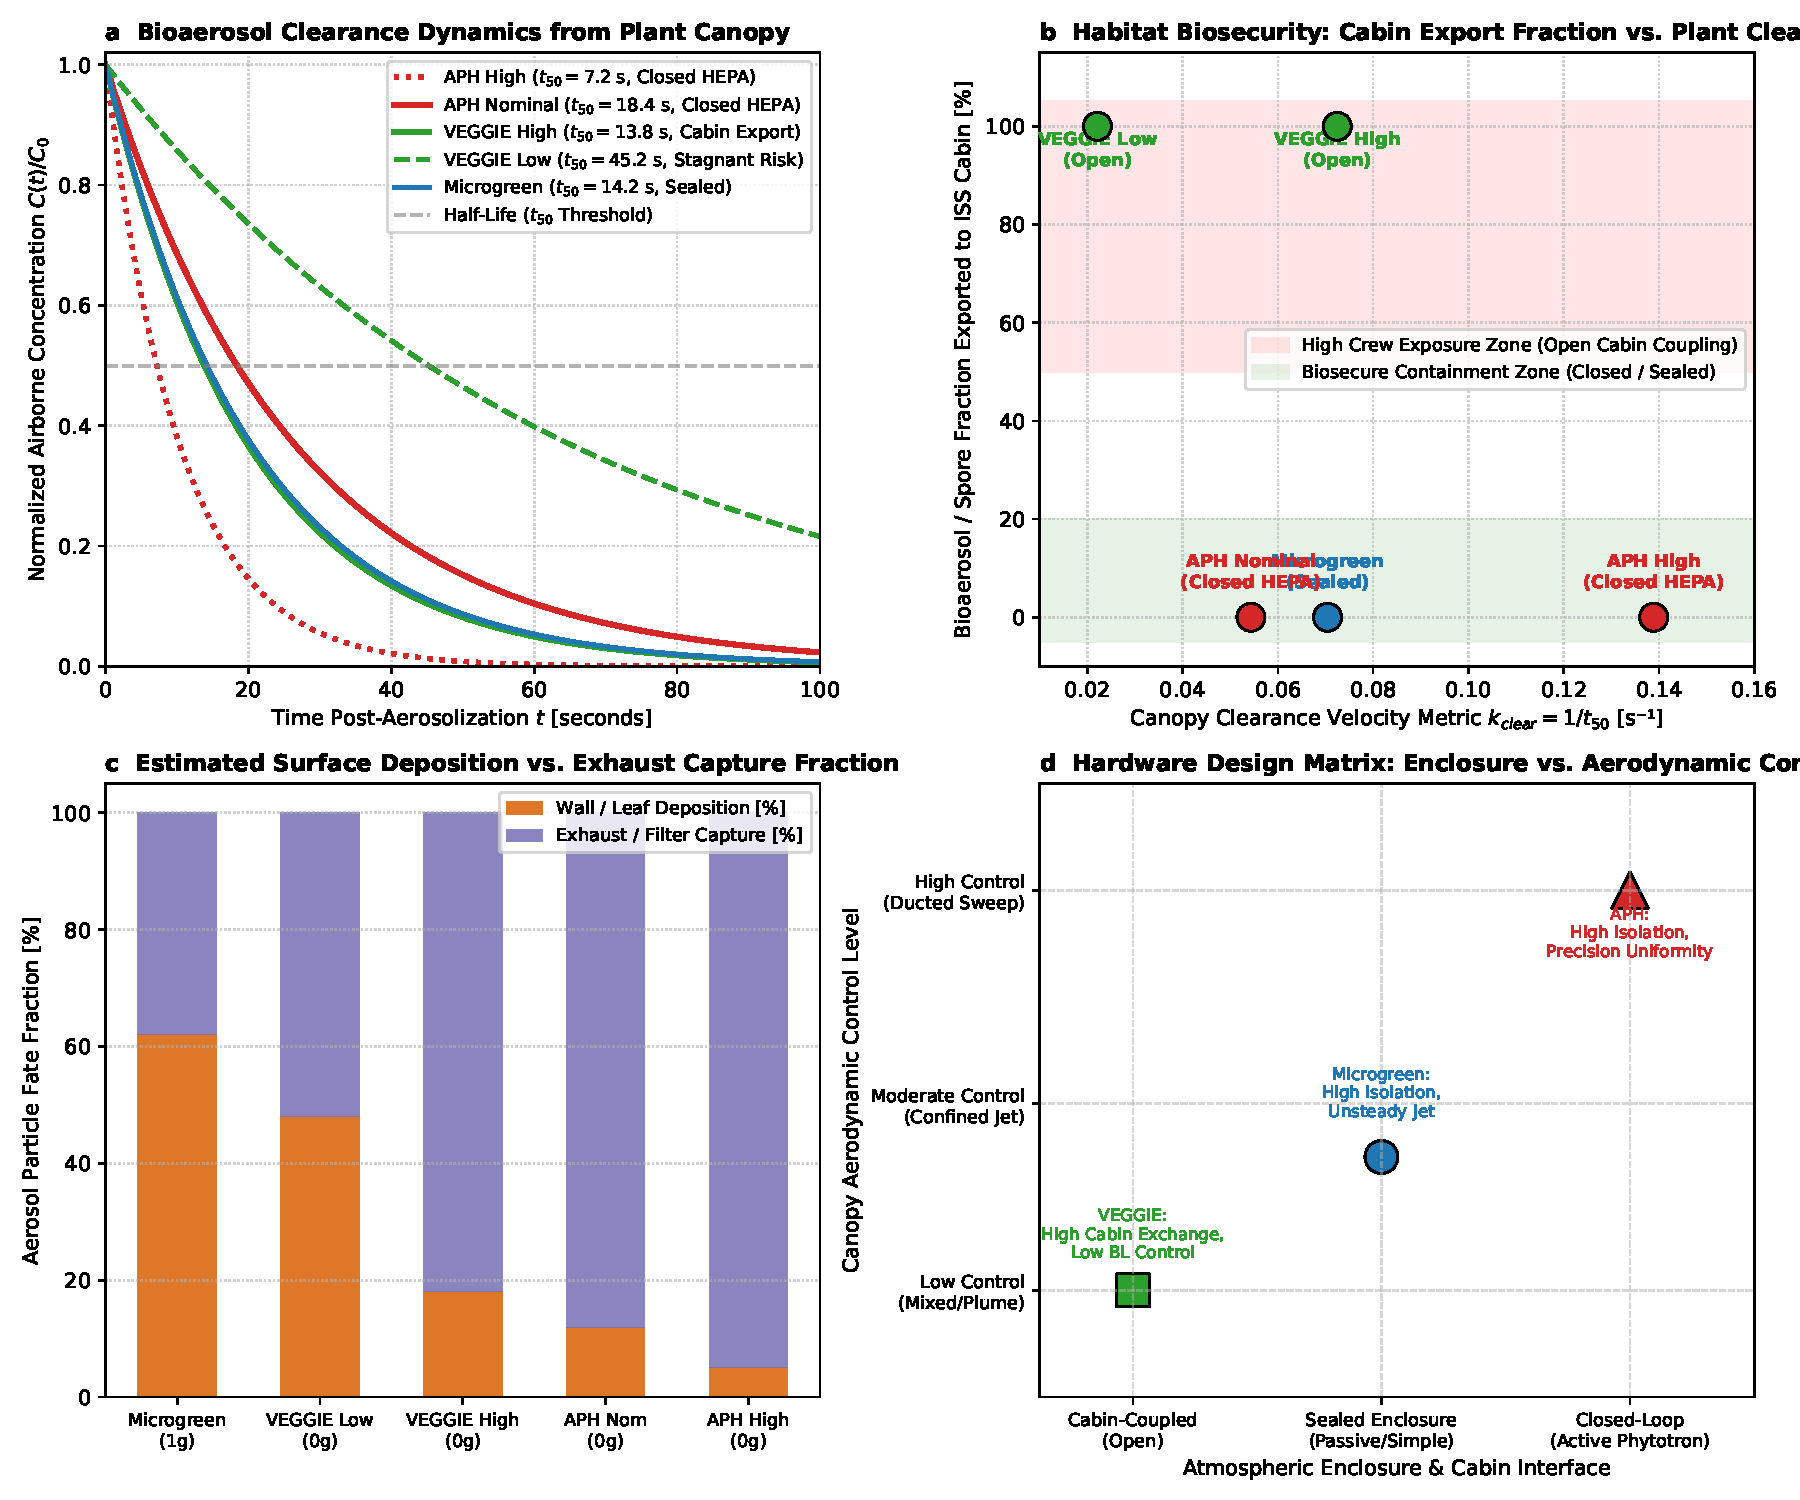
\includegraphics[width=\textwidth]{figures/output/Fig5_biosecurity_trades.pdf}
\caption{\textbf{Habitat biosecurity, bioaerosol clearance, and crew exposure trade space.} \textbf{a}, Transient bioaerosol clearance curves ($C(t)/C_0$) following spore release. \textbf{b}, Habitat biosecurity quadrant map: cabin export percentage vs. canopy clearance velocity metric ($k_{clear} = 1/t_{50}$). \textbf{c}, Aerosol particle fate: surface deposition vs. exhaust filtration. \textbf{d}, Two-dimensional architectural design matrix for spaceflight plant enclosures.}
\label{fig:fig5}
\end{figure*}

\begin{figure*}[t]
\centering
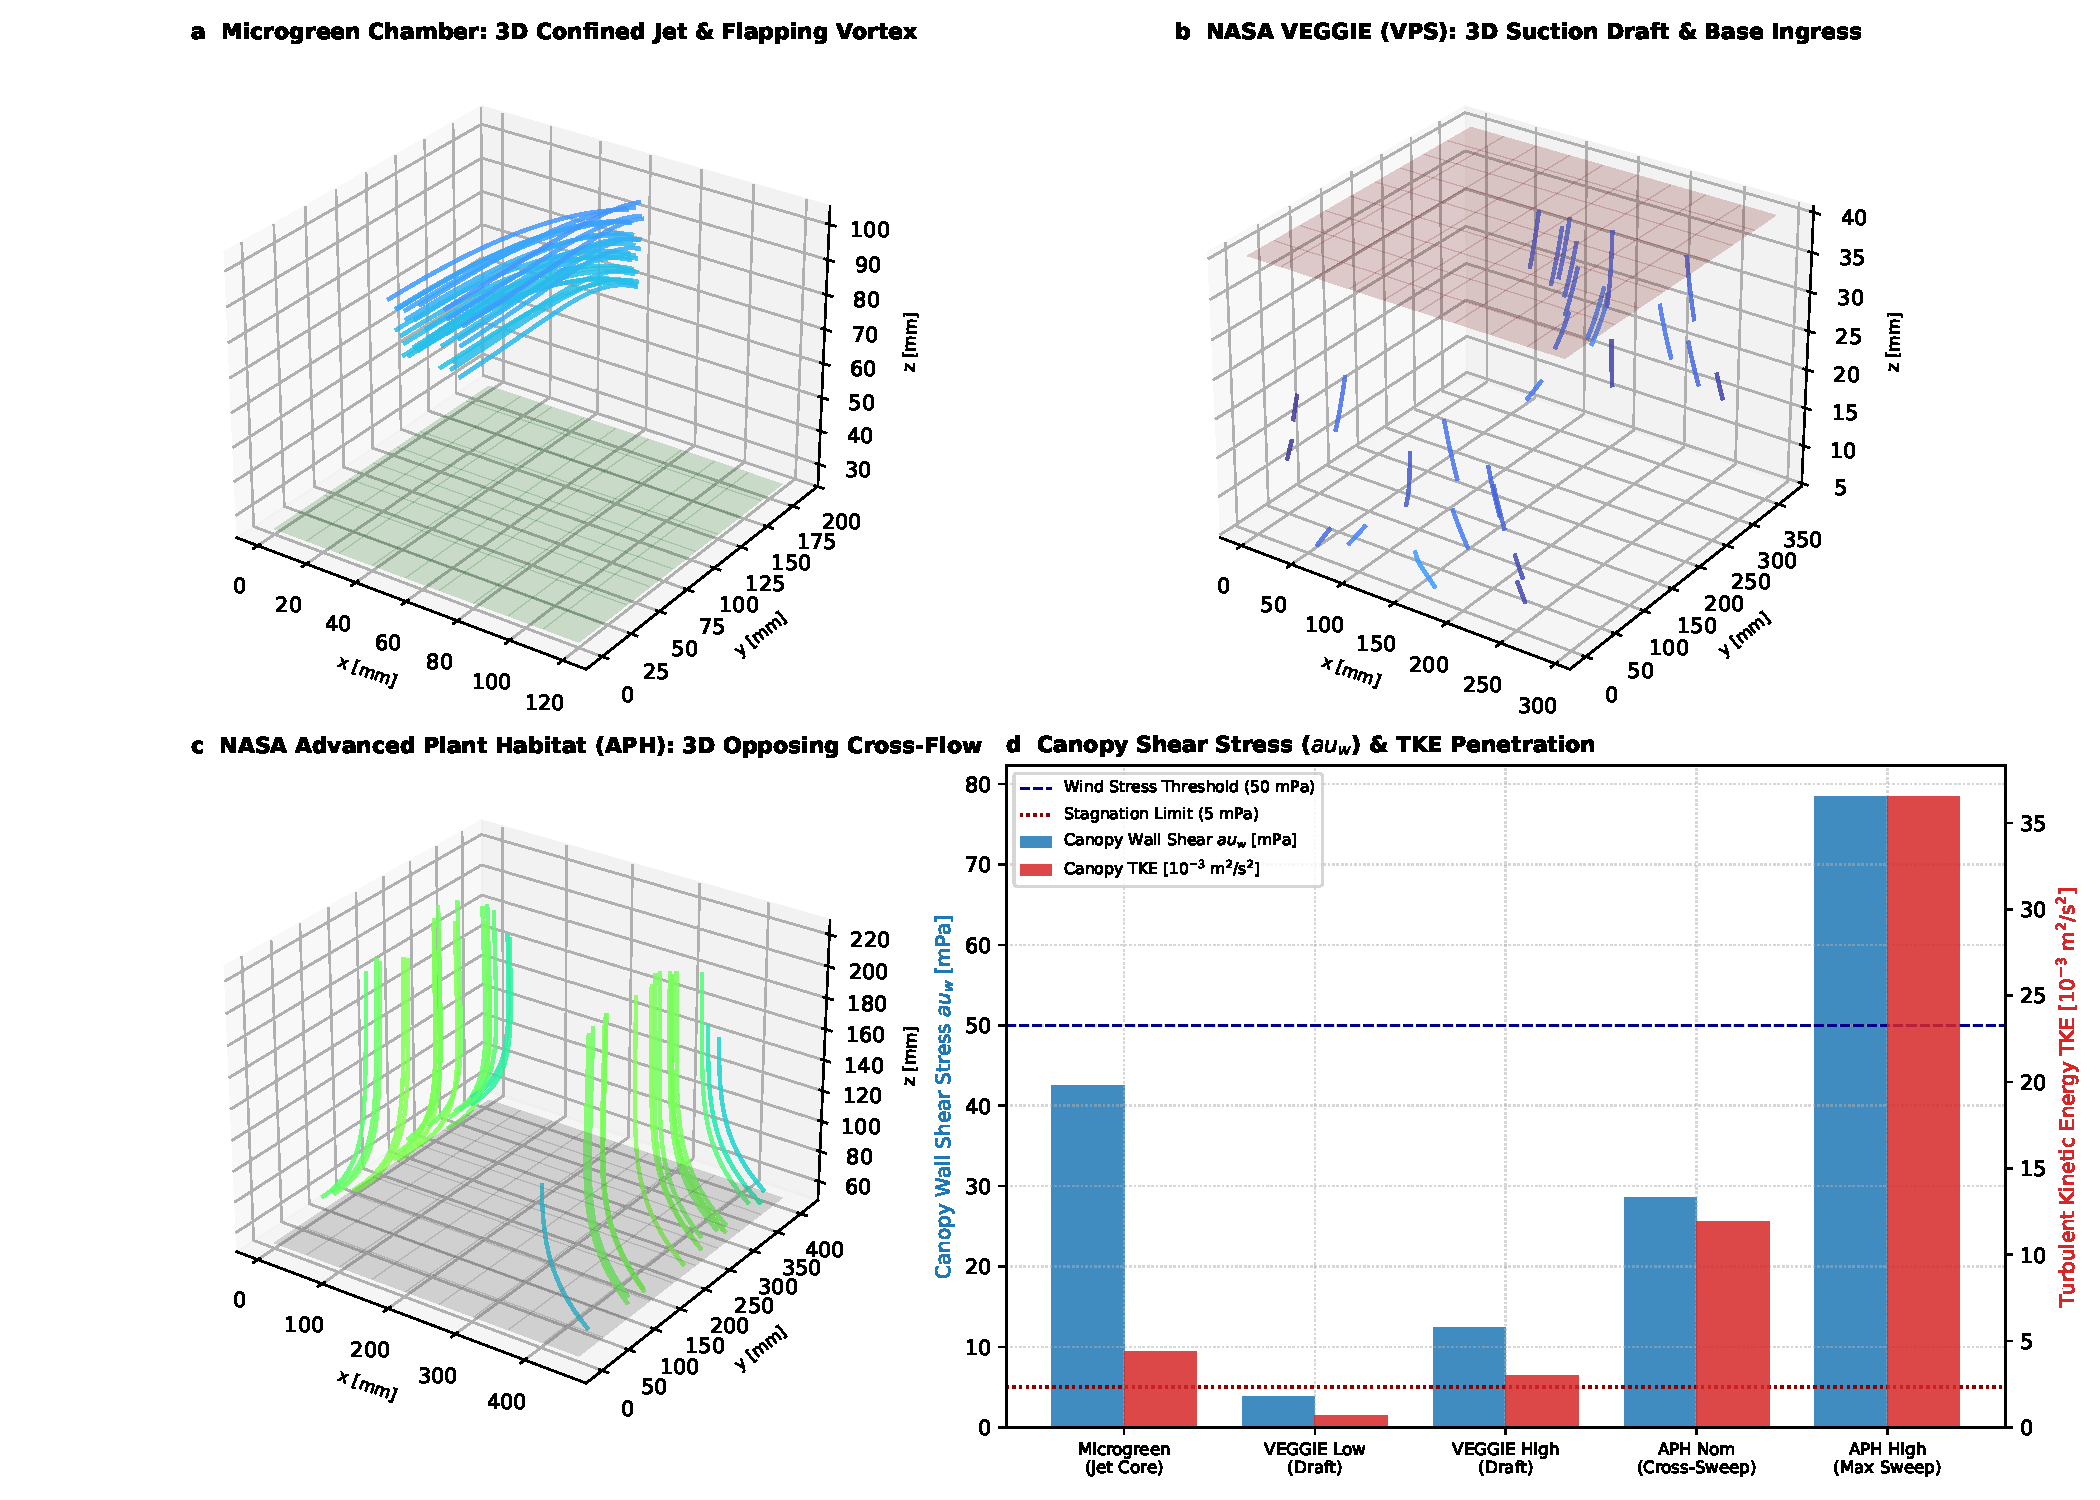
\includegraphics[width=\textwidth]{figures/output/Fig6_3d_flow_topologies.pdf}
\caption{\textbf{3D Spatial flow topologies, streamline ribbons, and canopy shear stress distributions.} \textbf{a}, Microgreen Chamber: 3D confined jet core and lateral recirculation secondary eddies. \textbf{b}, NASA VEGGIE: 3D suction draft streamlines drawn through 4 base slots toward the overhead exhaust fan. \textbf{c}, NASA Advanced Plant Habitat (APH): 3D opposing lateral cross-jets colliding over the Science Carrier and sweeping upward. \textbf{d}, Quantitative canopy wall shear stress ($\tau_w$) and turbulent kinetic energy (TKE) penetration across platforms.}
\label{fig:fig6}
\end{figure*}

\begin{figure*}[t]
\centering
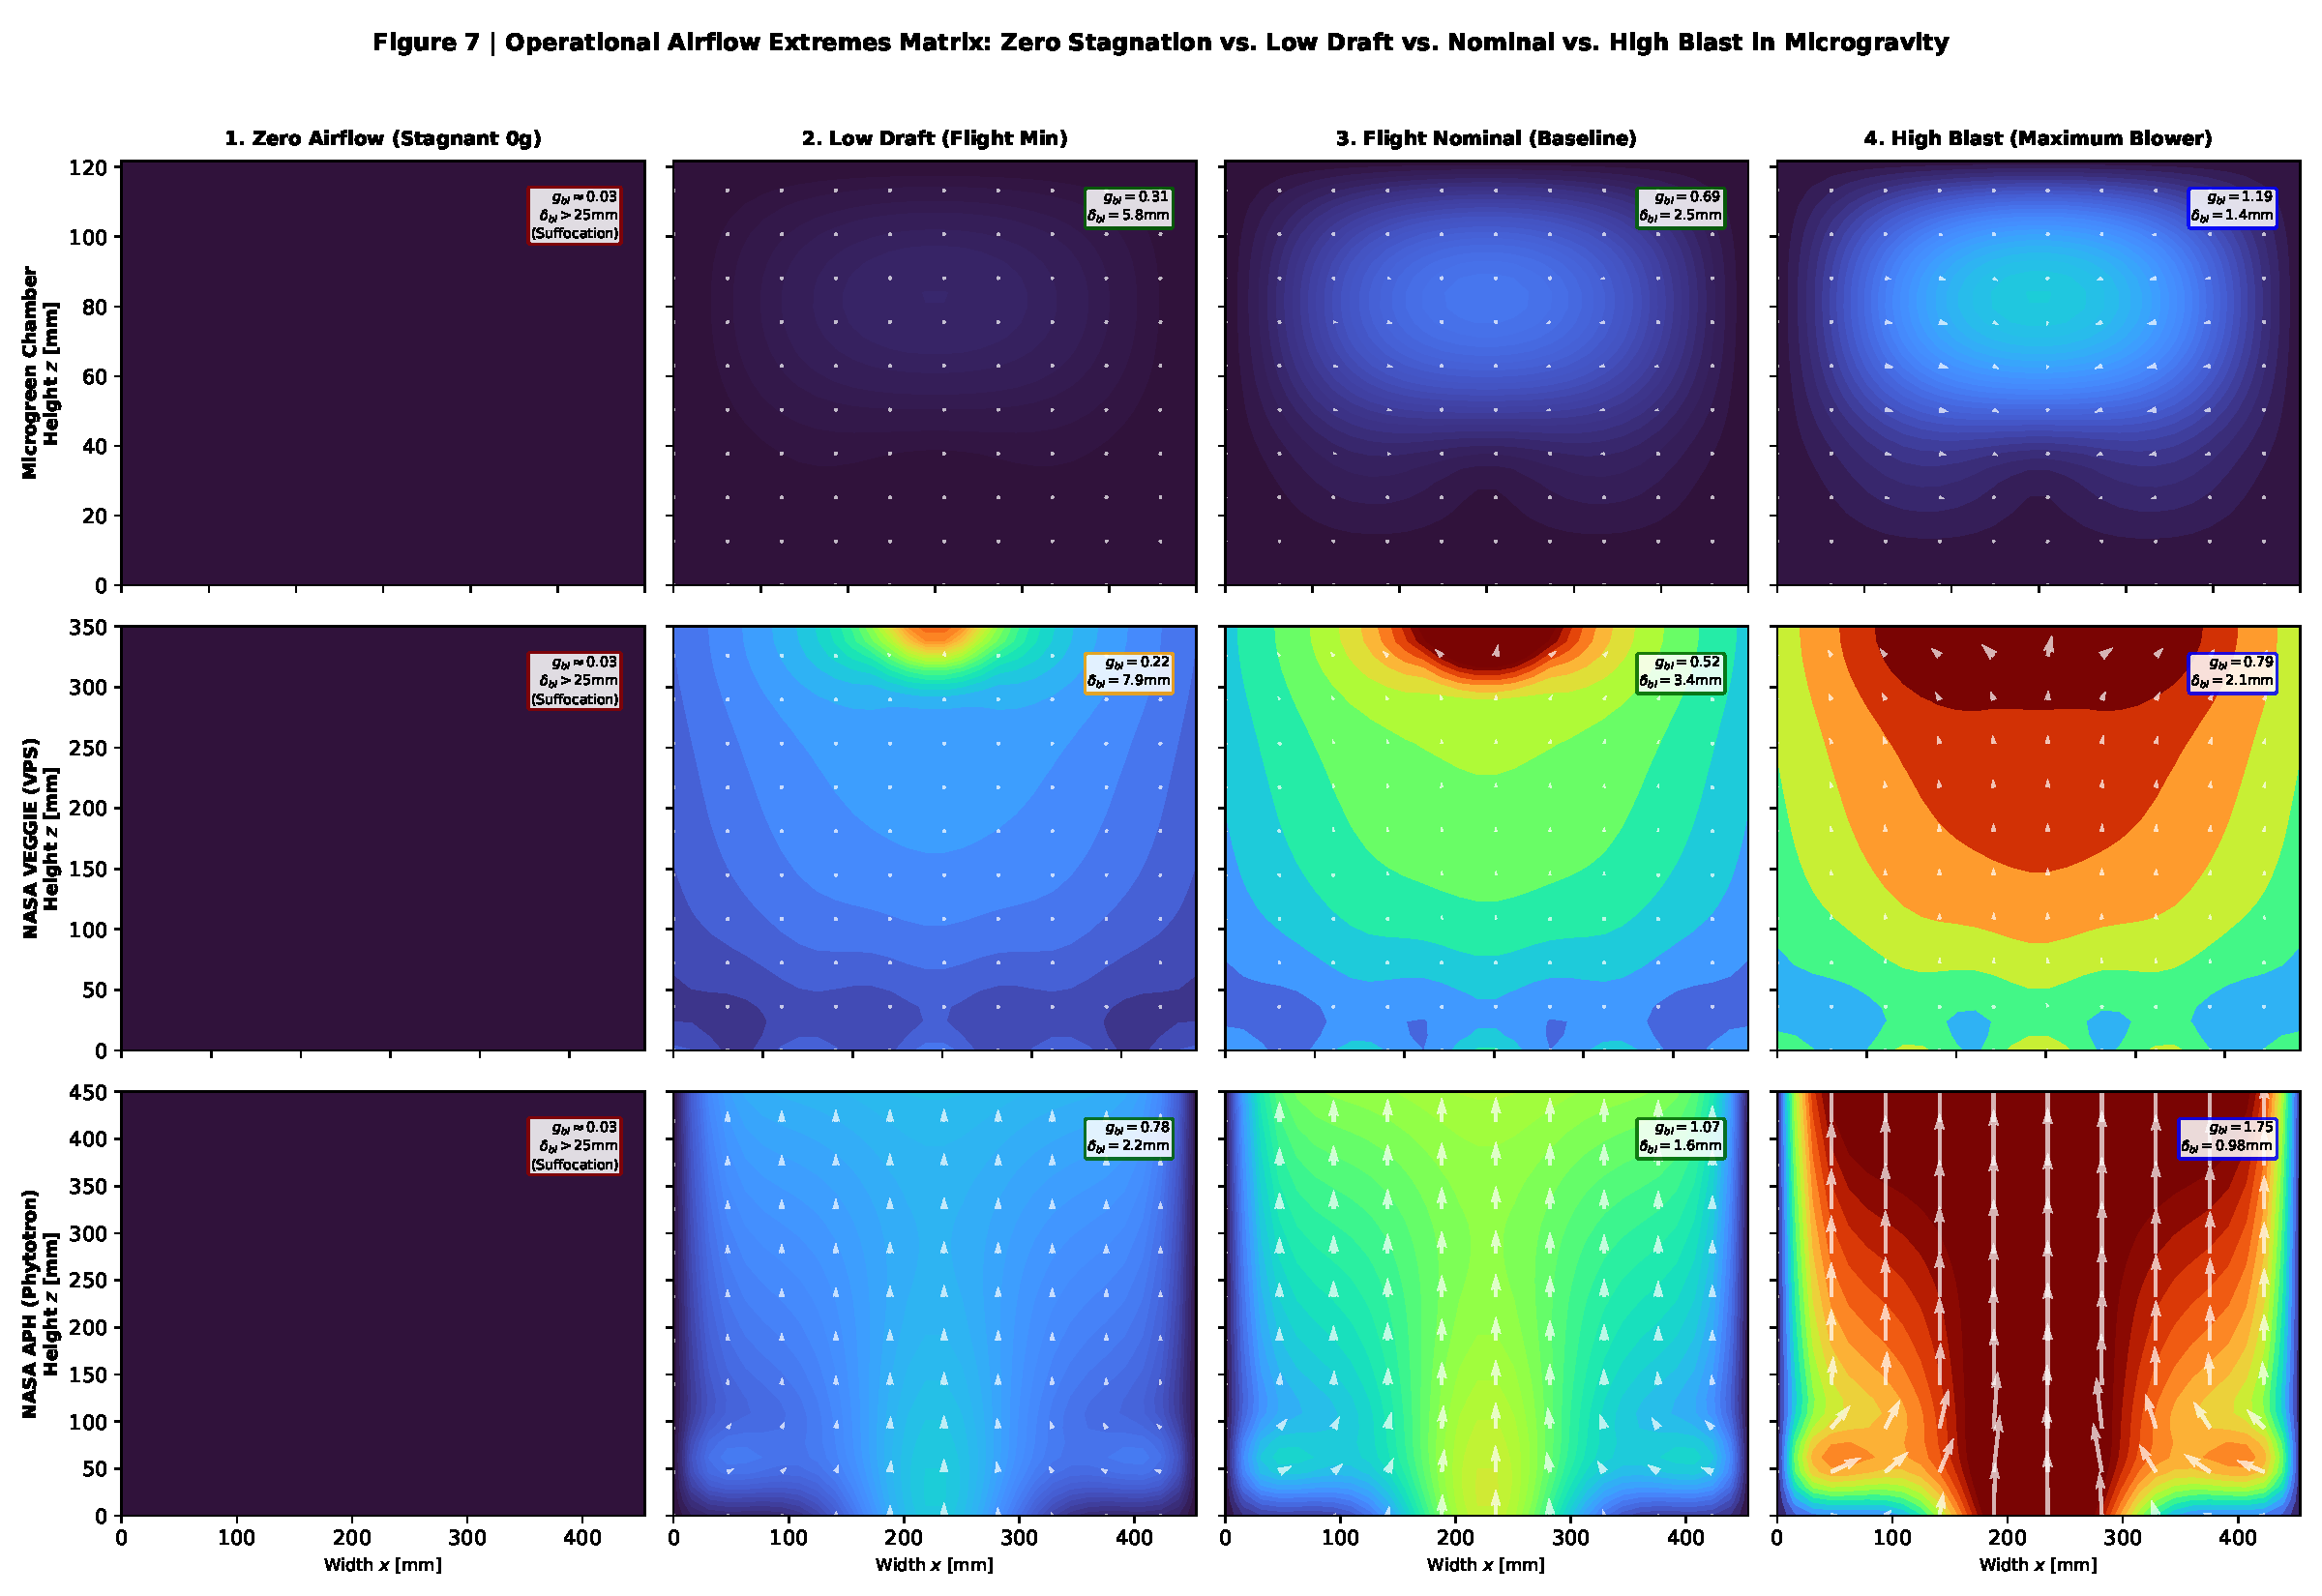
\includegraphics[width=\textwidth]{figures/output/Fig7_airflow_extremes.pdf}
\caption{\textbf{Operational airflow extremes and stagnation regimes across spaceflight plant growth hardware in microgravity.} Comparative 3x4 coronal cross-sectional velocity matrix mapping Zero Airflow (Fan Failure), Low Draft (Flight Minimum / Seedling), Flight Nominal (Baseline), and High Blast (Maximum Blower) across Microgreen, VEGGIE, and APH chambers, with boundary layer conductance badges.}
\label{fig:fig7}
\end{figure*}

\section*{Discussion}

Our multi-hardware CFD framework establishes that microgravity fundamentally alters the aerodynamic operating points of plant growth facilities, dismantling terrestrial design heuristics based on natural convection. The primary discoveries and their implications for space exploration include:

\subsection*{Buoyancy Collapse and the "Stratification Paradox"}
On Earth ($1\text{ g}$), overhead lighting systems inevitably generate stable thermal stratification when cold air is introduced from below or horizontally, creating a warm ceiling layer that damps vertical turbulent mixing. In microgravity ($0\text{ g}$), thermal buoyancy vanishes entirely ($Gr \to 0$). Consequently, forced air jets maintain their momentum trajectories without buoyant deflection, eliminating warm ceiling dead zones and improving turbulent kinetic energy penetration into the crop canopy. This "stratification paradox" explains why well-ducted chambers (like APH and the Microgreen Chamber) can achieve superior aerodynamic uniformity in space relative to ground controls.

\subsection*{The Vulnerability of Open / Low-Power Architectures}
VEGGIE's minimalist architecture was intentionally designed for low mass ($<20\text{ kg}$) and low power ($<100\text{ W}$), leveraging the ISS cabin as an infinite reservoir for temperature, $RH$, and $CO_2$ regulation~\cite{massa2017}. However, our CFD results demonstrate that this design creates severe aerodynamic compromises in microgravity. Without natural convection assisting the upward draft, the low-fan mode produces a $52.8\%$ stagnant volume fraction and drops boundary layer conductance to $0.219\text{ mol m}^{-2}\text{s}^{-1}$. To prevent fungal epidemics and physiological tipburn on long-duration missions (e.g., Artemis Base Camp or Mars transit), semi-open payloads must mandate continuous high-speed ventilation ($\ge0.15\text{ m/s}$ draft) or integrate local canopy oscillating stirrers.

\subsection*{Design Guidelines for Lunar and Martian Crop Modules}
On the Lunar ($0.166\text{ g}$) and Martian ($0.38\text{ g}$) surfaces, fractional gravity restores a partial buoyant convective regime ($Ri \approx 0.05 - 0.59$). For next-generation surface greenhouse modules (such as the LunarLeaf / Artemis BLSS concepts), our findings indicate that:
\begin{enumerate}
    \item \textbf{Opposing Cross-Flow Diffusers:} Dual opposing lower lateral supply slots (as demonstrated in APH) provide the highest air exchange efficiency ($\varepsilon_a > 45\%$) and lowest spatial non-uniformity across all gravities.
    \item \textbf{Decoupled Velocity Tuning:} Fan control should decouple bulk volumetric renewal ($\text{ACH} \sim 100 - 300\text{ h}^{-1}$) from local canopy shear velocity ($U_{canopy} \sim 0.3 - 0.6\text{ m/s}$) using recirculation diffusers, avoiding both boundary-layer suffocation ($U < 0.1\text{ m/s}$) and mechanical wind stress ($U > 1.2\text{ m/s}$).
    \item \textbf{Modular Biocontainment:} Enclosures should incorporate localized HEPA and activated-carbon scrubbing loops to prevent crop-to-crew pathogen transmission while eliminating volatile phytotoxins like ethylene.
\end{enumerate}

\section*{Methods}

\subsection*{Governing Equations and OpenFOAM Numerical Framework}
Simulations were executed within OpenFOAM v2606 (ESI-OpenCFD build) using finite-volume discretization of the compressible Navier-Stokes equations under the Low-Mach approximation:
\begin{equation}
    \frac{\partial \rho}{\partial t} + \nabla \cdot (\rho \mathbf{u}) = 0
\end{equation}
\begin{equation}
    \frac{\partial (\rho \mathbf{u})}{\partial t} + \nabla \cdot (\rho \mathbf{u} \mathbf{u}) = -\nabla p_{rgh} - (\mathbf{g} \cdot \mathbf{r})\nabla \rho + \nabla \cdot \left[ \mu_{eff} \left(\nabla \mathbf{u} + (\nabla \mathbf{u})^T - \frac{2}{3}(\nabla \cdot \mathbf{u})\mathbf{I}\right) \right] + \mathbf{S}_m
\end{equation}
\begin{equation}
    \frac{\partial (\rho h)}{\partial t} + \nabla \cdot (\rho \mathbf{u} h) + \frac{\partial (\rho K)}{\partial t} + \nabla \cdot (\rho \mathbf{u} K) = \nabla \cdot (\alpha_{eff} \nabla h) + \rho (\mathbf{u} \cdot \mathbf{g}) + S_h
\end{equation}
where $p_{rgh} = p - \rho \mathbf{g} \cdot \mathbf{r}$, $h$ is sensible enthalpy, $\mu_{eff} = \mu + \mu_t$, and $\alpha_{eff} = \frac{\mu}{Pr} + \frac{\mu_t}{Pr_t}$. 

Isothermal flow fields were solved using `simpleFoam` (steady SIMPLE) and `pimpleFoam` (transient PIMPLE), while thermal buoyancy cases utilized `buoyantSimpleFoam` and `buoyantPimpleFoam` with ideal gas equation of state ($perfectGas$) and Sutherland transport properties.

\subsection*{Turbulence Modeling and Boundary Layer Resolution}
Turbulence was modeled using the two-equation Shear Stress Transport ($k\text{-}\omega\text{ SST}$) model~\cite{menter1994}, which combines $k\text{-}\omega$ formulation in the inner boundary layer with $k\text{-}\epsilon$ behavior in the free stream. Wall boundaries employed continuous wall functions (`nutkWallFunction`, `kqRWallFunction`, `omegaWallFunction`), ensuring accurate wall shear stresses across the $y^+ \sim 1 - 5$ regime.

\section*{Data and Code Availability}
All raw mesh files, OpenFOAM case dictionaries, generated STL surfaces, CSV summary tables, interactive 3D WebGL visualizations, and 4D animated simulation files are available on GitHub at \url{https://github.com/HenryEwald/microgreen-chamber-cfd}.

\bibliographystyle{naturemag}
\bibliography{references}

\end{document}
